

\subsection{Usefulness Analysis}
\label{cp6:usefulness}


Having compared the correctness of manual and tool-assisted tasks as well 
as the amount of overlap between text identified as relevant by the participants and 
text automatically identified by our tool, we turn to the question of 
whether the highlights shown by the tool were considered helpful. 
For that, we analyze participants' ratings and the feedback that they 
provided at the end of our experiment.







\paragraph{\textbf{Metrics.}}

To investigate the usefulness of the highlights shown by our tool, we asked participants to indicate in a 5 points Likert scale whether the highlights
of each artifact were helpful to correctly accomplish their assigned task (Figure~\ref{fig:experiment-rating}). We aggregate individual responses to measure how useful was 
the tool in assisting developers complete each task in our experiment, plotting responses using a diverging stacked bar chart~\cite{spence2001info-viz}.



\paragraph{\textbf{Data.}}


Participants produced a total of 197 ratings representing the usefulness of the highlights shown by our tool in the artifacts inspected.
On average, we collected 65 responses per task and 7 responses per artifact.  
These values do not match the exact number of participants and artifacts in our experiment since some participants did skip this part of 
the survey for their own reasons.


We also obtained written feedback from 19 out of the 24 participants in our experiment. This was divided on feedback for the tasks (24 data points)
or the experiment itself (15 data points). We use this feedback to discuss potential threats or ways to improve the tool in sections~\ref{cp6:threats} 
and~\ref{cp6:summary}, respectively.



% \subsubsection{Results}


\paragraph{\textbf{Results.}}


From all the ratings collected on the  usefulness of the text automatically identified and shown by our tool, 40\% of them agreed that the highlights were useful, 
25\% neither agreed nor disagreed on their usefulness, and 35\% that indicated that they were \textit{not} usefulness.
Similar to how we presented results on correctness, we analyze usefulness ratings on a per task basis.  




Figure~\ref{fig:usefulness-by-task} shows participants' ratings aggregated for each task. 
Participants indicated that the highlights shown for the \texttt{titanic} task were the most useful. 
ratings for this task might support our observations on its correctness as well as on our comparison of manual and tool identified text. 
Notably, one participant indicated that highlights for this task assisted them in identifying essential function arguments needed to perform the task---``\textit{some of the highlights were useful when there were clear special meanings to particular function arguments like as\_index=True}''.


In contrast, participants indicated that the highlights for the \texttt{distances} task were on its majority not useful. 
For example, one participant pointed out that, in the \texttt{geopy} API documentation, there were no highlights in 
a section were they would have expected otherwise---``\textit{I also went to the documentation $>$ Distance, but surprisingly nothing was highlighted}''.




\begin{figure}
    \centering
    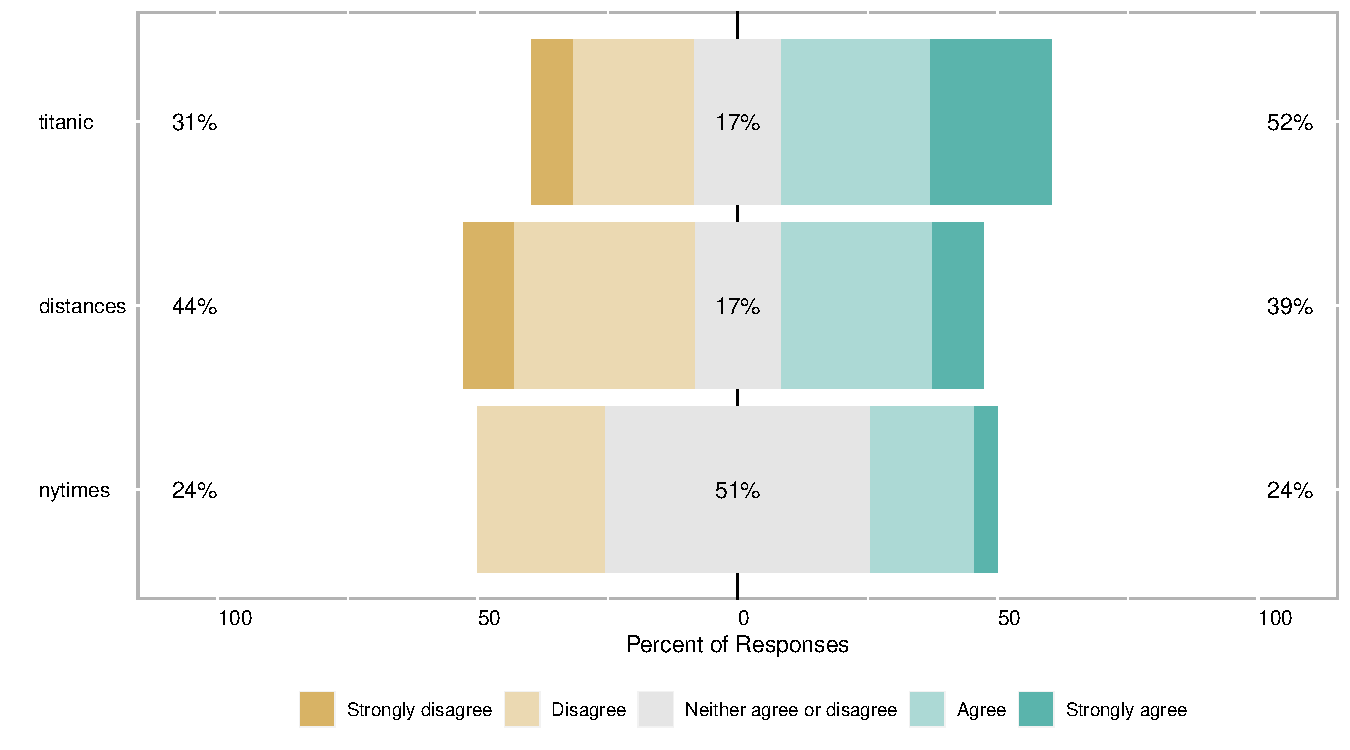
\includegraphics[width=.9\textwidth]{cp6/usefulness_overall.pdf}
    \caption{Diverging stacked plot of the usefulness of the text automatically identified for each task}
    \label{fig:usefulness-by-task}
\end{figure}




Surprisingly, when we look at the ratings per type of artifact (Figure~\ref{fig:usefulness-by-artifact-type}), API documents had the most useful highlights.






\begin{figure}
    \centering
    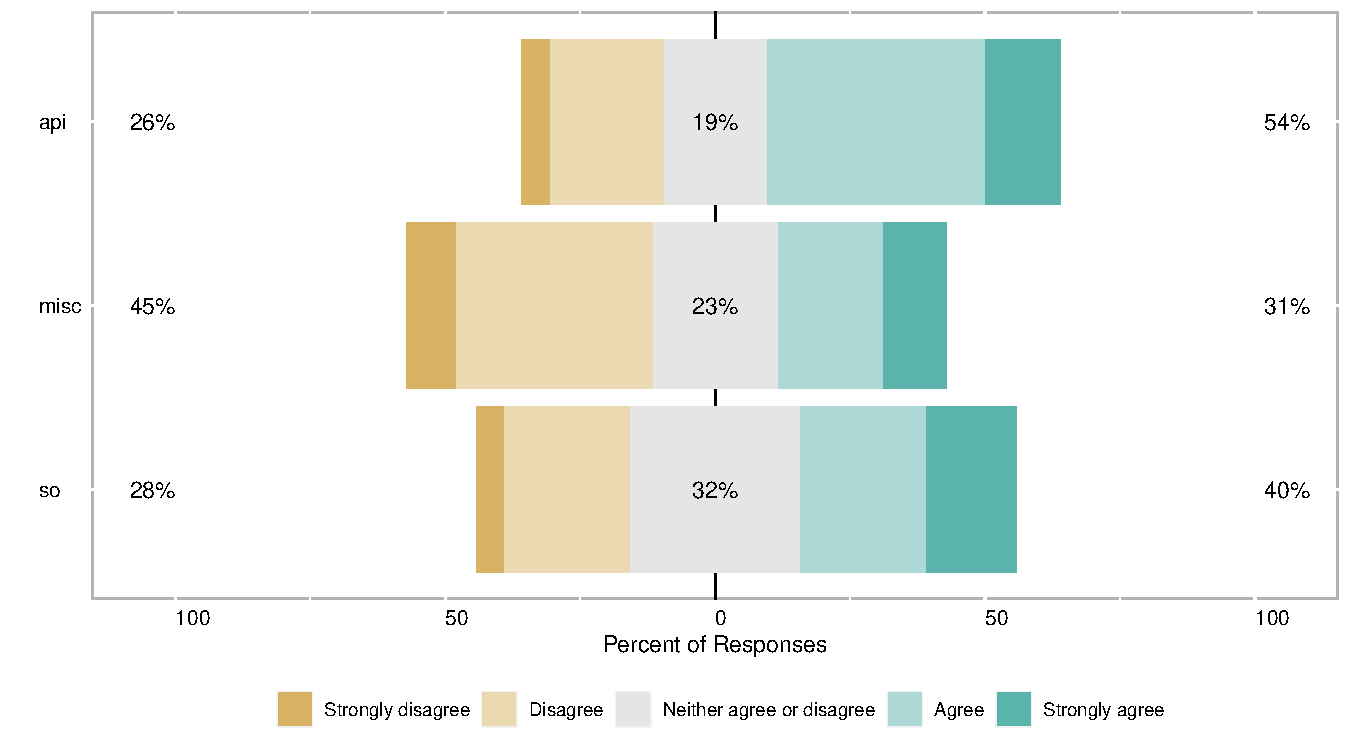
\includegraphics[width=.9\textwidth]{cp6/usefulness_per_type.pdf}
    \caption{Diverging stacked plot of the usefulness of the text automatically identified for each type of artifact}
    \label{fig:usefulness-by-artifact-type}
\end{figure}









